\chapter{Progettazione}

In questo capitolo viene descritta l'architettura del progetto, derivata dall'analisi dei requisiti.

\section{Architettura del sistema \label{arch}}
Il sistema è costituito da due macro-parti:
\begin{itemize}
 \item un server che costituisce il punto di centralizzazione;
 \item un insieme di dispositivi embedded che dialogano con il server.
\end{itemize}
I dispositivi embedded hanno un comportamento locale, ovvero gestito individualmente da ognuno, e uno globale, cioè che richiede interazioni con il server centrale.
Quest'ultima parte costituisce l'elemento di maggiore criticità, in quanto la quasi totalità delle interazioni si concentra sul server.
\\Per far fronte ai requisiti di performance, reattività, scalabilità, facilità di gestione e interoperabilità, si è scelto di adottare REST come strategia di comunicazione, poiché possiede le seguenti caratteristiche fondamentali:
\begin{itemize}
 \item la comunicazione è di tipo client-server come richiesto;
 \item la comunicazione è \textit{stateless}, ovvero non necessita della memorizzazione di alcun contesto client sul server;
 \item consente di implementare facilmente un'architettura scalabile a livelli con nodi di commutazione intermedi;
 \item è universalmente riconosciuta e supportata, basandosi su HTTP + TCP + IP.
\end{itemize}
\subsection{Nota sull'utilizzo dei Raspberry Pi}
Nella realizzazione di questo progetto si è scelto di utilizzare dispositivi Raspberry Pi come dispositivi embedded, in quanto largamente noti e utilizzati.
Da qui in avanti si parlerà indifferentemente di ``Raspberry'' e ``dispositivi embedded'', tuttavia anche altre tipologie di sistemi embedded possono essere utilizzate senza problemi, compresi i microcontrollori (al fine di ridurre i costi).
L'utilizzo dei sistemi Raspberry comunque presuppone la presenza di un sistema Linux sottostante, per cui da ora in poi si considererà questa ipotesi tecnologica.


\section{Progettazione Server}
Il server (o il cluster di server, a seconda dell'implementazione) dovrà fornire i seguenti servizi:
\begin{itemize}
 \item un server web che fornirà un'interfaccia centralizzata per l'invio di comandi ai Raspberry;
 \item una servlet che si occuperà di ricevere attraverso un'interfaccia REST messaggi provenienti dai Raspberry, fungendo da intermediaria con il database;
 \item un Time Series DBMS sul quale sono registrati i cambiamenti di stato segnalati dalla servlet;
 \item un sistema di generazione di statistiche e grafici basati sui dati contenuti nel Time Series DBMS;
 \item un DBMS relazionale (opzionale) per l'archiviazione di credenziali d'accesso e indice dei Raspberry che fanno parte del sistema;
\end{itemize}

\subsection{Tipologia del server}
Poiché la parte server ricopre un ruolo centrale nel sistema, è necessario valutare le alternative a disposizione, per poi scegliere quella più idonea:
\begin{itemize}
 \item acquisto di server dedicati;
 \item server cloud di tipo \textit{Infrastructure as a Service} (IaaS);
 \item server cloud di tipo \textit{Platform as a Service} (PaaS).
\end{itemize}
\paragraph{Acquisto di server dedicati}
Una prima possibilità è quella di acquistare server dedicati.
Questa modalità prevede un investimento iniziale maggiore e richiede di sostenere direttamente tutti i costi di gestione nel tempo, quali elettricità, sistemi di raffreddamento, gruppi di continuità, sostituzione dei componenti difettosi e impiego di personale specializzato.
Questo potrebbe essere un problema nel caso in cui i server da gestire (compresi anche quelli non collegati a questo sistema) fossero pochi, in quanto i costi difficilmente sarebbero ammortizzati.
E inoltre, le necessità in termini di prestazioni in un sistema di questo tipo possono essere molto variabili con il crescere del sistema stesso.
Una città che optasse per l'acquisto di server dedicati, dovrebbe necessariamente acquistarli con prestazioni sovradimensionate rispetto all'utilizzo iniziale, in previsione del carico a regime.
Questa opzione è consigliabile nel caso la città sia già in possesso dei server utilizzati per altri scopi.
\paragraph{Server cloud IaaS}
Una seconda possibilità è quella di affidarsi ad un provider di servizi cloud \textit{IaaS}, che consentirebbe di spostare i costi di gestione e manutenzione del server all'interno di un datacenter.
Sarebbe comunque necessario un sistemista per l'installazione e la manutenzione regolare del software sul server, a partire dal sistema operativo.
Inoltre, diventa possibile un rapido ridimensionamento delle risorse hardware allocate ai server, per far fronte alle richieste crescenti nel tempo (ipotizzando che i Raspberry vengano installati in maniera progressiva), riducendo i costi iniziali.
\paragraph{Server Cloud PaaS}
Utilizzando server cloud \textit{PaaS}, l'astrazione si sposta di un livello verso l'alto, in quanto si rimuove la necessità di gestire il sistema operativo, focalizzandosi solo sui servizi.
In questo modo si semplifica ulteriormente la gestione, a costo di una minore configurabilità dei servizi (si è molto più soggetti all'offerta del provider scelto).
\paragraph{Scelta finale}
Valutate le alternative, si è deciso di scartare l'acquisto di server dedicati, poiché si è ritenuto più importante consentire il rapido ridimensionamento delle risorse hardware dedicate, garantendo scalabilità.
Tra le due soluzioni \textit{IaaS} e \textit{PaaS} si è scelta la prima, in quanto le attuali proposte \textit{Paas} sul mercato sono state ritenute troppo limitanti nelle funzionalità per il tipo di sistema che si vuole realizzare.
Inoltre, anche in base al requisito di interoperabilità, si è ritenuto opportuno evitare soluzioni ``vendor specific''.

\subsection{Server Web}
Il server web centrale è utilizzato dagli operatori per modificare la configurazione dei Raspberry e per eseguirne la manutenzione.
L'utilizzo di tale interfaccia è saltuario, e difficilmente più operatori la utilizzano concorrentemente.
Per questo motivo le risorse necessarie a fornire questo servizio sono contenute e non è necessario adottare strategie particolari: è quindi sufficiente un normale web server.
La comunicazione con i Raspberry avviene tramite interfaccia REST, dove l'interfaccia web in esecuzione sul server centrale costituisce il client e ogni Raspberry costituisce un server.
Ulteriori dettagli sul funzionamento della comunicazione tra il server web e i Raspberry sono descritti nella progettazione della parte Raspberry (sezione \ref{seq-diagram-webserver}).

\subsection{Time Series DBMS}
Analizzando i dati prodotti dai Raspberry, risaltano i seguenti aspetti:
\begin{itemize}
 \item ne vengono prodotte grandi quantità in relativamente poco tempo;
 \item la dimensione del singolo messaggio è molto contenuta;
 \item sono fortemente time-oriented, ovvero l'accesso avviene prima di tutto in base al tempo (timestamp) in cui sono stati registrati.
\end{itemize}
Per questi motivi si è valutata l'opportunità di archiviarli su un database non relazionale, sia per motivi di performance, sia per ottimizzare la componente time-oriented degli accessi.
I \textit{time series database} (TS-DBMS) sono stati ideati precisamente per venire incontro a queste esigenze.
Un TS-DBMS consente di creare, enumerare, aggiornare, eliminare ed organizzare serie temporali.
L'organizzazione può essere gerarchica e includere metadati associati.
È possibile eseguire operazioni su intere serie di dati come la moltiplicazione, l'addizione e combinare più serie di dati in un'unica serie, applicando trasformazioni.
I dati possono essere filtrati basandosi su pattern temporali, valori di soglia minimi e massimi o altre funzioni matematiche.
\paragraph{Formato dei dati}
I dati memorizzati sul TS-DBMS sono legati da un rapporto di cardinalità uno a uno con quelli relativi ai messaggi inviati dai Raspberry e contengono:
\begin{itemize}
 \item tipologia dell'evento;
 \item host che ha generato l'evento;
 \item area geografica (eventualmente quartiere) in cui si trova l'host;
 \item azione eseguita;
 \item intensità luminosa impostata sui lampioni;
 \item valore di luminosità registrato dalla fotoresistenza;
 \item timestamp.
\end{itemize}
Sulla base di questi dati sarà possibile costruire statistiche e grafici per analizzare i pattern di utilizzo e valutare strategie per migliorare l'efficienza energetica complessiva nella città.

\subsection{Servlet}
Al fine di garantire scalabilità e sicurezza, i Raspberry non comunicano direttamente con il DBMS, ma si appoggiano ad un intermediario, che ha lo scopo di ricevere ed elaborare i messaggi dei Raspberry per poi inviarli al DBMS.
Le comunicazioni in ingresso e in uscita dalla servlet seguono il paradigma REST, ovvero i Raspberry contattano la servlet attraverso la sua interfaccia REST e lo stesso fa la servlet nei confronti del TS-DBMS.
È possibile eseguire multiple istanze della servlet su server diversi per distribuire il carico e introdurre ridondanza.
\paragraph{Interfaccia REST}
La servlet espone l'interfaccia REST descritta in figura \ref{API REST SERVLET}, utilizzata dai Raspberry.
L'entry point \textit{changeLightIntensity} è utilizzato per notificare un avvenuto cambio di intensità luminosa (a causa delle policy impostate sul Raspberry); \textit{changePolicy} notifica l'avvenuta reimpostazione delle policy (a causa dell'intervento di un operatore attraverso l'interfaccia web); \textit{notifyError} notifica un problema di funzionamento.
\begin{figure}[ht]
	\centering
	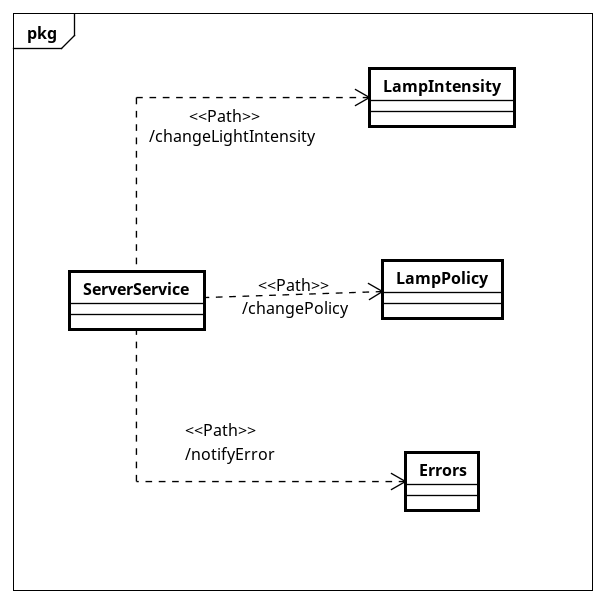
\includegraphics[scale=.8]{figure/Class_Diagram_Server_REST.png}
	\caption{API REST Servlet \label{API REST SERVLET}}
\end{figure}
\paragraph{Diagramma di sequenza}
In figura \ref{SEQ RPI TO SERVER} sono mostrate le interazioni tra Raspberry e servlet, e tra servlet e TS-DBMS.
\begin{figure}[h!]
	\centering
	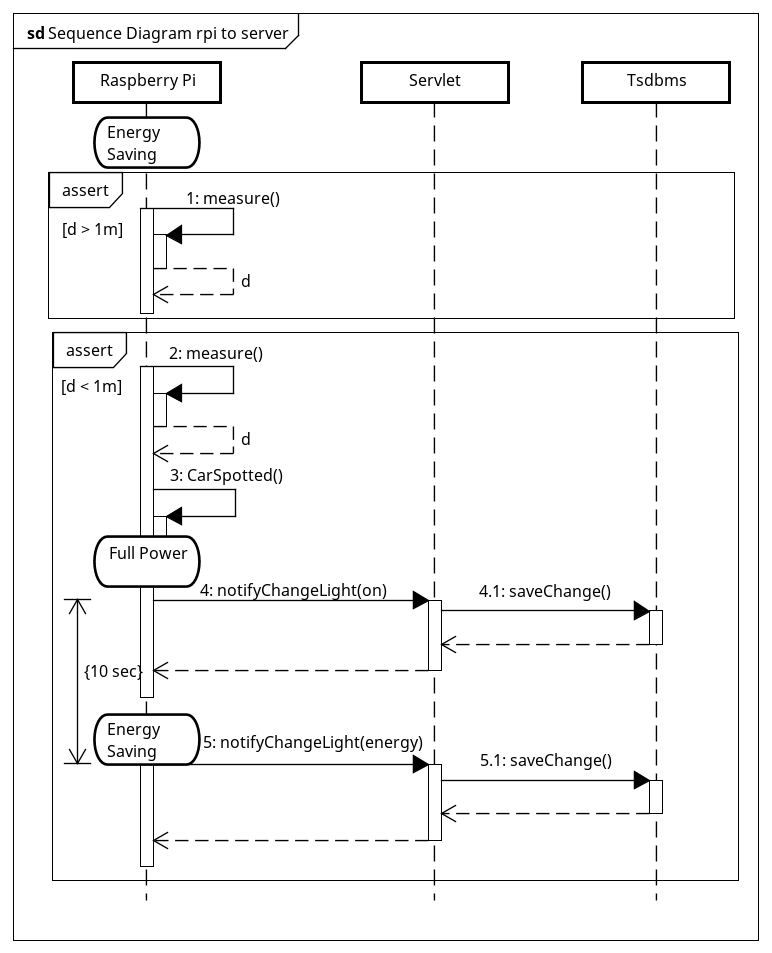
\includegraphics[scale=.63]{figure/Sequence_Diagram_rpi_to_server.png}
	\caption{Diagramma di sequenza delle comunicazioni tra Raspberry, servlet e TS-DBMS \label{SEQ RPI TO SERVER}}
\end{figure}

\subsection{Sistema di generazione di statistiche e grafici}
La consultazione diretta dei dati memorizzati nel TS-DBMS può non essere user-friendly, e sicuramente non praticabile dall'utente medio.
Vale la pena quindi di garantire una modalità di fruizione maggiormente accessibile.
In particolare, si vuole rendere possibile la generazione di statistiche e grafici basati sui dati contenuti nel TS-DBMS.
Il sistema dovrà essere estendibile, in modo che i grafici non siano cablati all'interno del software, ma l'utente abbia modo di costruirli personalizzandoli in base alle proprie esigenze.
Una volta che tali grafici saranno costruiti, saranno fruibili anche dall'utente medio; l'utente avanzato sarà in grado di generare dinamicamente i grafici di cui ha bisogno.

\subsection{DBMS relazionale}
In aggiunta al TS-DBMS, si può valutare anche l'utilizzo di un DBMS relazionale per mantenere alcune informazioni semi-statiche o generate in quantità di gran lunga inferiori rispetto a quelle memorizzate nel TS-DBMS, quali:
\begin{itemize}
 \item l'anagrafica dei Raspberry dislocati sul territorio;
 \item le credenziali di accesso ai singoli Raspberry;
 \item eventuali dati statistici sintetici relativi allo storico dei guasti.
\end{itemize}


\section{Progettazione Raspberry}
Il sistema Raspberry fornisce le seguenti funzionalità:
\begin{itemize}
 \item rilevamento dell'illuminazione ambientale con il sensore di luce;
 \item rilevamento della presenza di automobili con i sensori di prossimità;
 \item illuminazione di ogni singolo lampione in base alle politiche locali;
 \item programma principale che gestisce il web server REST e l'invio delle statistiche al server.
\end{itemize}
Essendo il software dei Raspberry composto da diverse parti tra loro autonome e concorrenti, si è scelto di utilizzare il paradigma ad attori, un modello computazionale concorrente a più alto livello rispetto alla gestione manuale dei thread.
In questo modo ogni componente logica è un attore e la comunicazione avviene esclusivamente tramite scambio di messaggi.

\subsection{Interfaccia REST}
Come spiegato in precedenza nell'architettura del sistema (sezione \ref{arch}), i Raspberry devono offrire un'interfaccia REST (figura \ref{API REST RPI}) che permetta di:
\begin{itemize}
	\item ottenere la configurazione attuale di un determinato lampione;
	\item modificare le policy di accensione e spegnimento;
	\item modificare le configurazioni per il risparmio energetico;
	\item permettere di iniziare e concludere una fase di debug per poter fare prove sul funzionamento dei lampioni;
	\item comunicare ai Raspberry vicini il sopraggiungere di un mezzo sulla carreggiata (comportamento locale ai Raspberry).
\end{itemize}
\begin{figure}[ht!]
	\centering
	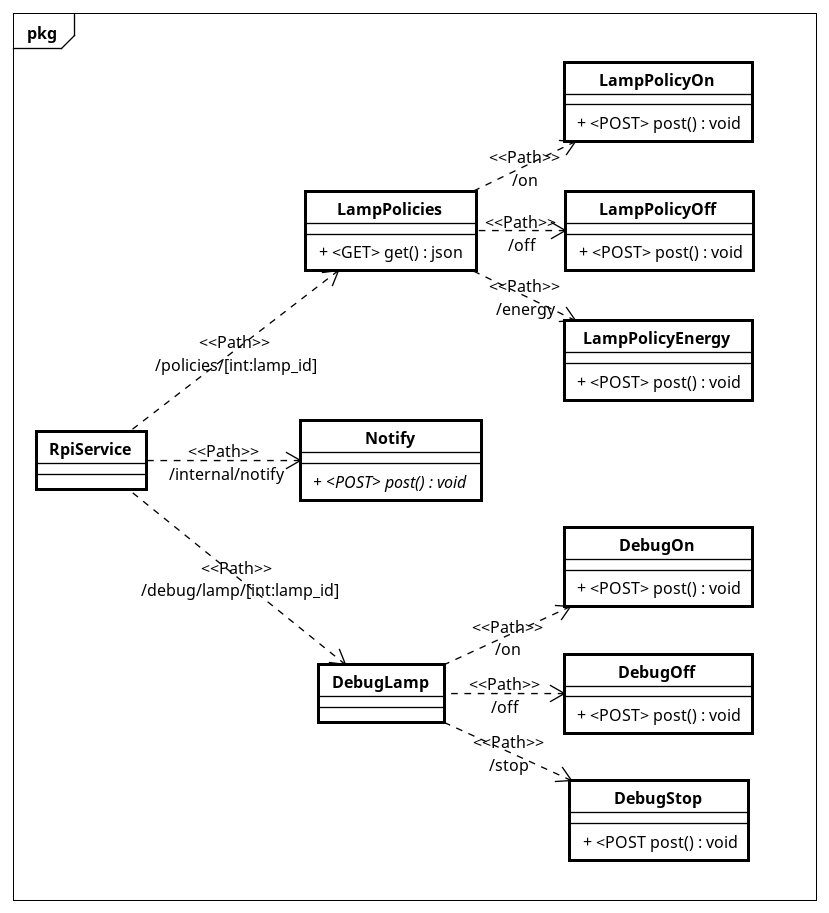
\includegraphics[scale=.62]{figure/Class_Diagram_Rpi_REST.png}
	\caption{API REST Raspberry \label{API REST RPI}}
\end{figure}

\subsection{Policy del sistema}
L'eventuale illuminazione di un lampione è regolata da policy stabilite in maniera centralizzata e modificabili anche mentre il sistema è in esecuzione.
A meno che non venga rilevato il passaggio di un'auto o di un livello di intensità luminosa eccedente il limite impostato nelle policy, l'unico fattore che viene considerato per l'accensione dei lampioni è l'orario corrente.
\paragraph{Macchina a stati finiti}
Per mostrare il comportamento del sistema riguardante le policy temporali si è utilizzata la macchina a stati finiti semplificata in figura \ref{FSM POLICY}.
Inizialmente i lampioni partono dallo stato \textit{off} e, se l'orario corrente (rappresentato dalla variabile \textit{t}) è successivo all'orario impostato per la policy \textit{on}, allora il lampione passerà allo stato \textit{on}.
In seguito, quando l'orario supererà la soglia di \textit{policy energy on}, il lampione andrà in modalità risparmio energetico passando allo stato \textit{energy saving}.
In tale modalità l'intensità luminosa sarà ridotta fino a quando non viene rilevato un mezzo in transito sulla carreggiata.
Alla fine del periodo di risparmio energetico, impostato da \textit{policy energy off}, il lampione tornerà allo stato di partenza, spegnendosi.
\begin{figure}[ht]
	\centering
	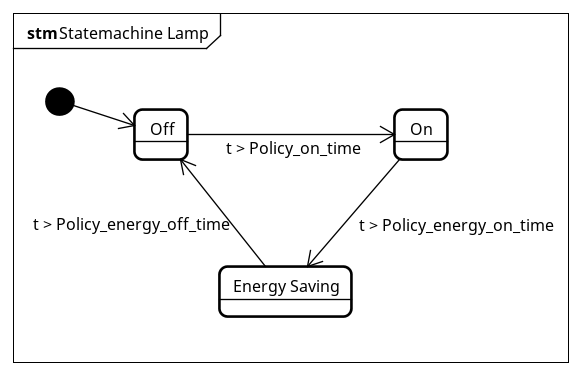
\includegraphics[scale=.8]{figure/Statemachine_Lamp.png}
	\caption{Finished State Machine relativo alle policy del sistema \label{FSM POLICY}}
\end{figure}

\subsection{Controllo presenza auto}
Questa parte si occupa di controllare la presenza di eventuali mezzi in transito.
Utilizzando un sensore di prossimità, periodicamente viene calcolata la distanza tra il sensore e l'ostacolo più vicino per valutare se un'auto possa essere in transito in quel momento sulla carreggiata.
\paragraph{Comportamento sensore di prossimità}
Per la rappresentazione dell'architettura è stato scelto di utilizzare una ``Finished State Machine''.
Come si può notare in figura \ref{FSM CAR}, all'avvio di \textit{Ultrasonic} vengono avviati due comportamenti concorrenti: il primo ha il compito di aggiungere e rimuovere i lampioni interessati ad essere notificati del passaggio di auto; il secondo si occupa di fare la rilevazione della distanza tra il sensore e l'oggetto in quel momento più vicino.
Partendo dallo stato \textit{waiting}, se è presente almeno un attore, viene effettuata una lettura di distanza e, se il valore è maggiore della distanza tra il sensore e la larghezza della carreggiata, attende per qualche millisecondo e poi ritorna nello stato \textit{waiting}.
Se invece il valore è minore della larghezza della carreggiata, significa che è stato rilevato un mezzo in transito e quindi vengono notificati tutti i lampioni attualmente in lista.
Dopo aver aspettato qualche secondo, ritorna allo stato iniziale \textit{waiting}.
\begin{figure}[ht!]
	\centering
	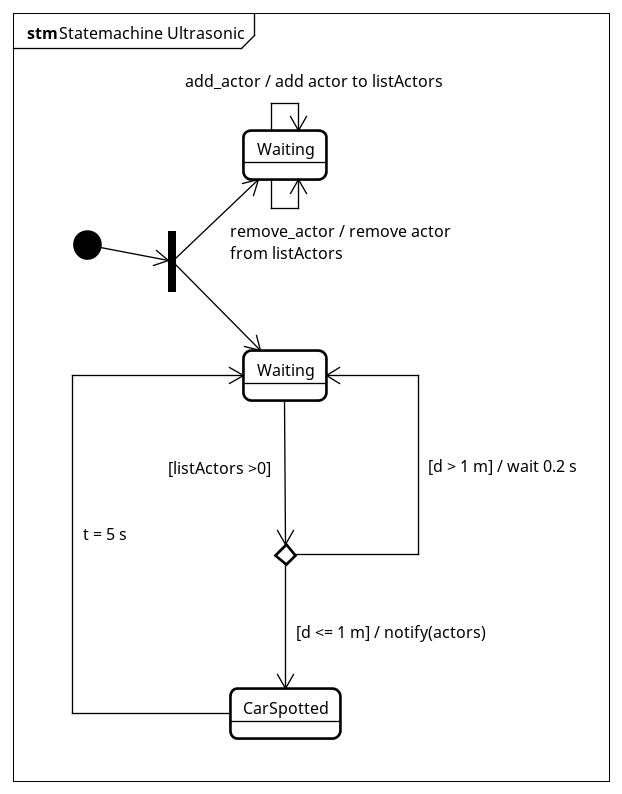
\includegraphics[scale=.75]{figure/Statemachine_Ultrasonic.png}
	\caption{Finished State Machine riguardante la parte di controllo presenza auto \label{FSM CAR}}
\end{figure}
\paragraph{Cambiamento di stato dei lampioni}
Utilizzando il diagramma di sequenza in figura \ref{SD CAR}, è stato rappresentato il cambio di stato da parte di due lampioni dal risparmio energetico alla piena potenza dopo la rilevazione di un'auto in transito.
Inizialmente i lampioni si trovano nello stato di risparmio energetico e viene effettuata una misurazione da parte del sensore di prossimità che restituisce la lettura rappresentata da \textit{d}.
Successivamente viene eseguita una seconda lettura: questa volta la distanza rilevata si assume equivalga a meno della soglia impostata come necessaria, e quindi che sia stata rilevata un'automobile.
Per questo vengono notificati entrambi i lampioni, i quali, dopo un intervallo di tempo calcolato tramite la moltiplicazione tra una costante e il proprio identificativo, passano in modalità di piena potenza per permettere all'automobilista di percorrere la strada in sicurezza.
\begin{figure}[ht!]
	\centering
	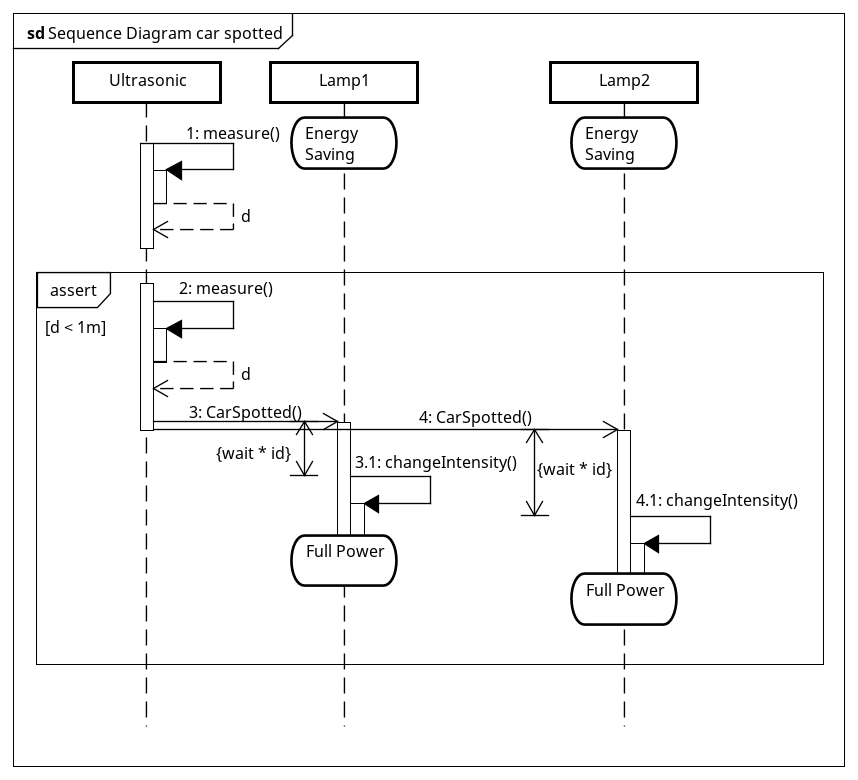
\includegraphics[scale=.59]{figure/Sequence_Diagram_car_spotted.png}
	\caption{Comunicazione tra il sensore ad ultrasuoni e i lampioni rappresentata tramite un Sequence Diagram \label{SD CAR}}
\end{figure}
\paragraph{Notifica ai dispositivi vicini}
Quando viene rilevato un mezzo in transito sulla carreggiata e tutti i lampioni di un determinato Raspberry si sono accesi, verrà comunicato ai dispositivi embedded successivi al proprio che un mezzo sta per sopraggiungere.
Come scritto in precedenza, le notifiche saranno messaggi di tipo REST.
Notificare i vicini è necessario per due motivi:
\begin{itemize}
	\item i lampioni successivi si potranno accendere tempestivamente;
	\item nel caso si giungesse ad un incrocio, verranno notificati tutti i dispositivi embedded relativi alle strade dell'intersezione.
\end{itemize}

\subsection{Controllo luminosità ambientale}
Questa parte si occupa di controllare l'intensità luminosa ambientale e di notificare i lampioni in modo che possano accendersi o spegnersi se il valore di luminosità fosse maggiore o minore di una certa soglia impostata nelle loro policy.
\paragraph{Architettura}
Per la rappresentazione dell'architettura è stato scelto di utilizzare una Finished State Machine.
In figura \ref{FSM PR} viene mostrato come inizialmente siano presenti due comportamenti concorrenti.
Come per il caso del controllo della presenza di auto, anche qui il primo è responsabile della gestione della lista dei lampioni da notificare;
il secondo si occupa di eseguire la lettura dell'intensità luminosa e di notificare ogni lampione presente nella lista.
\\Il secondo parte dallo stato \textit{waiting} ed esegue una lettura se la lista dei lampioni non è vuota.
In seguito invia la lettura effettuata a tutti gli elementi della lista e aspetta nello stato \textit{prMeasured} per qualche secondo.
Infine torna nello stato \textit{waiting}.
\begin{figure}[ht!]
	\centering
	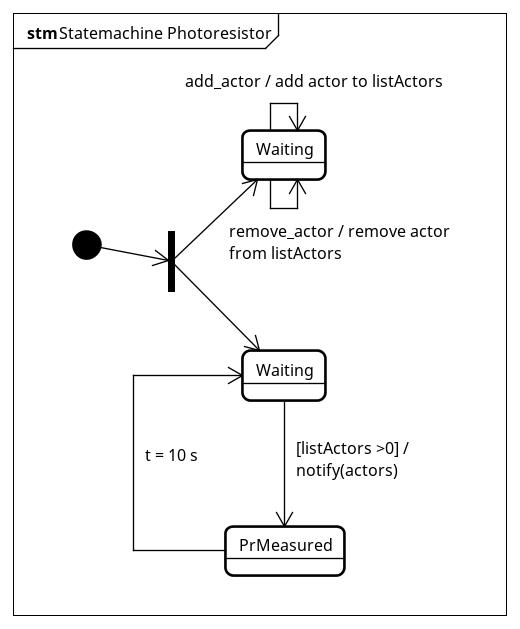
\includegraphics[scale=.8]{figure/Statemachine_Photoresistor.png}
	\caption{Finished State Machine riguardante la lettura della luminosità ambientale \label{FSM PR}}
\end{figure}

\subsection{Web Server}
Il web server deve poter comunicare con i Raspberry dislocati sul territorio per poter ottenere e modificare le impostazioni locali di ogni dispositivo.
Per questo si mette in comunicazione con i Raspberry utilizzando le loro interfacce REST.
\paragraph{Diagramma di sequenza \label{seq-diagram-webserver}}
Come si può vedere in figura \ref{SD WEB} per la rappresentazione della comunicazione tra il web server e i Raspberry è stato utilizzato un diagramma di sequenza.
Nel primo esempio viene mostrata la richiesta da parte di un utente per ricevere le policy relative al lampione numero 1 da un determinato Raspberry.
Il web server utilizzando un URL prestabilito effettua una GET.
Il Raspberry ottiene le policy in formato JSON dal lampione 1 e restituisce tali informazioni al web server, che successivamente le mostrerà all'utente.
\\Il secondo esempio è simile al primo, con la differenza che in questo caso l'utente intende effettuare una modifica alla policy on del lampione 1.
Quindi il web server questa volta invierà una POST al Raspberry di competenza, il quale notificherà del cambiamento il lampione coinvolto.
Infine, verrà mostrato all'utente l'esito di tale operazione.
\begin{figure}[ht]
	\centering
	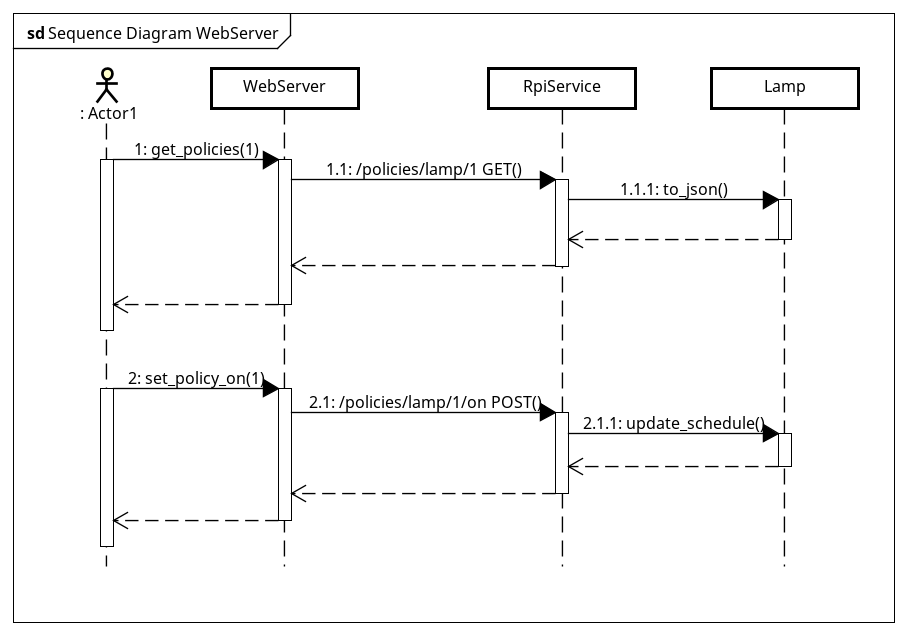
\includegraphics[scale=.55]{figure/Sequence_Diagram_WebServer.png}
	\caption{Sequence diagram per la comunicazione tra web server e Raspberry Pi \label{SD WEB}}
\end{figure}


\section{Deployment}
Essendo i vari dispositivi Raspberry necessariamente dislocati sul territorio, si può agire su di essi solo variando il numero di lampioni controllati da ognuno.
Per quanto riguarda il lato server, invece, è possibile disaccoppiare i servizi su più server, al fine di migliorare le prestazioni e la ridondanza.
Verranno ora descritti i principali metodi di deployment.
Sono naturalmente possibili soluzioni intermedie.

\subsection{Centralizzazione totale}
Una soluzione è quella di installare tutti i servizi su un unico server (figura \ref{DD CENT}).
Questo minimizza i costi di deployment, ma limita le prestazioni e porta alla costituzione di un pericoloso ``single point of failure''.
La riduzione delle prestazioni può non essere un problema nel caso di sistemi di dimensioni ridotte, mentre lo è su sistemi più estesi.
La costituzione di un ``single point of failure'', invece, è da tenere bene in considerazione, in quanto un guasto sul server potrebbe causare problemi a tutto il sistema.
\begin{figure}[ht]
	\centering
	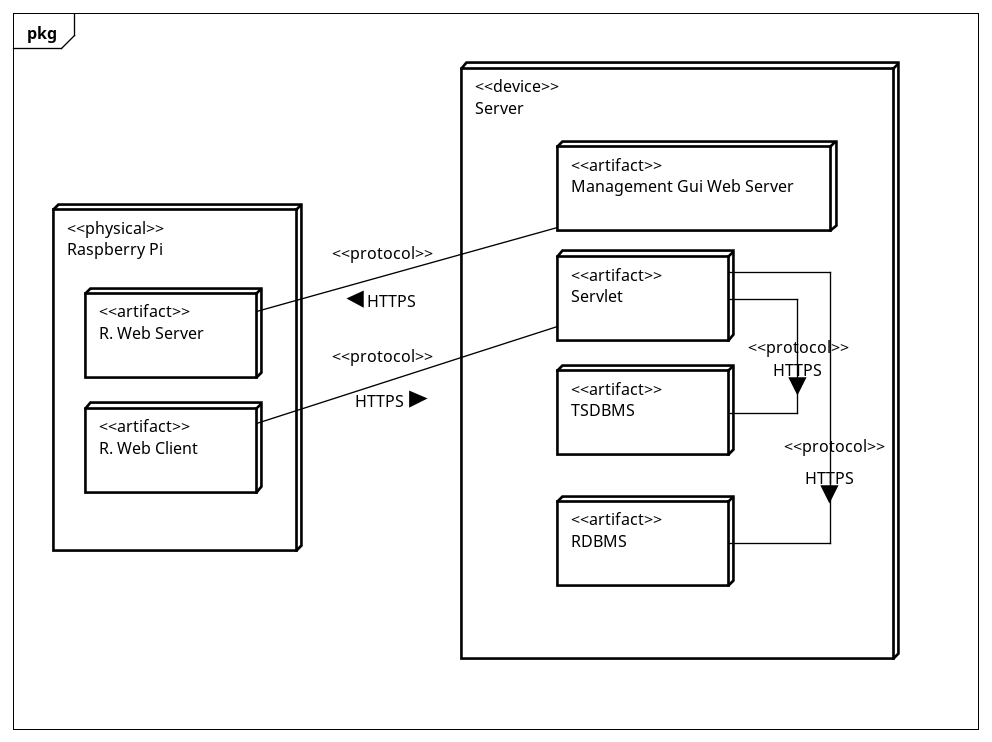
\includegraphics[scale=.5]{figure/Deployment_Diagram_2.png}
	\caption{Diagramma di deployment (server centralizzato) \label{DD CENT}}
\end{figure}

\subsection{Distribuzione}
La soluzione più scalabile e consigliata è quella di installare i vari servizi su server separati (figura \ref{DD DIST}): questo porta ad un forte incremento delle prestazioni, e riduce l'impatto derivante da eventuali guasti.
\begin{figure}[ht]
	\centering
	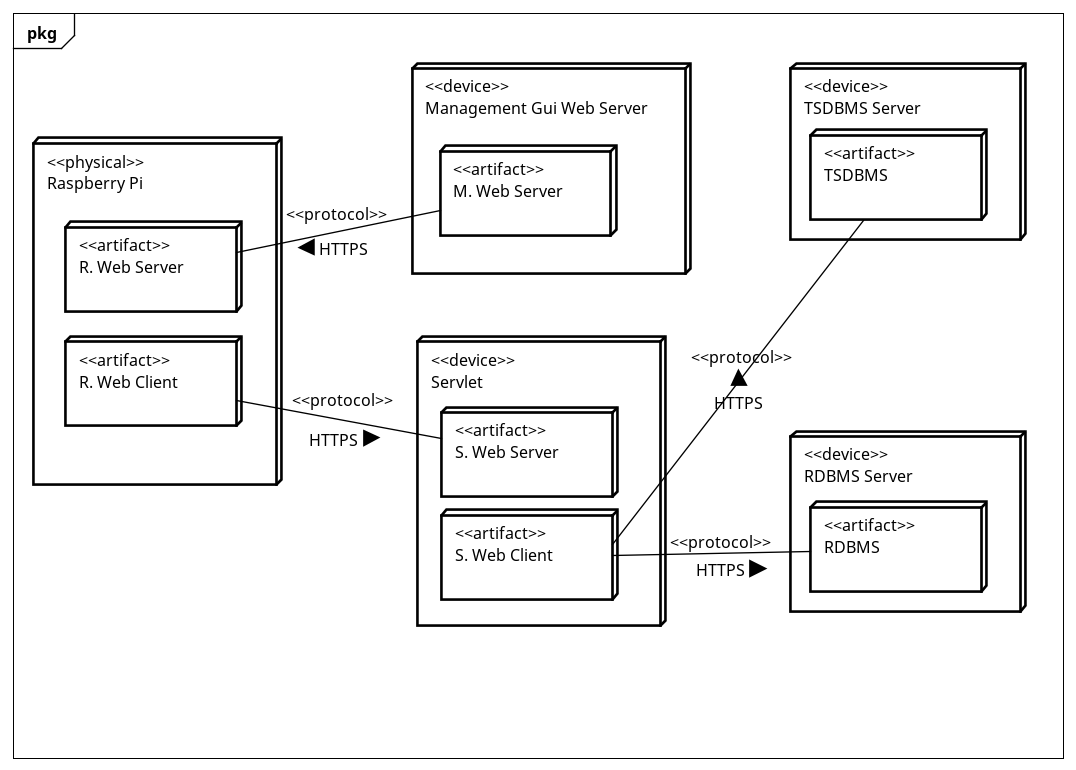
\includegraphics[scale=.45]{figure/Deployment_Diagram_1.png}
	\caption{Diagramma di deployment (server distribuito) \label{DD DIST}}
\end{figure}

\subsection{Layer di smistamento}
Un'ulteriore soluzione prevede di utilizzare un layer di smistamento, installando più istanze della servlet su server diversi (figura \ref{DD LAYERED}).
In questo modo il nucleo del traffico non convergerebbe direttamente sul server centrale, ma verrebbe smistato precedentemente, facendo attività di load balancing.
Inoltre, in caso di problemi con un'istanza specifica della servlet, solo i Raspberry direttamente collegati ad essa ne risentirebbero.
\begin{figure}[ht]
	\centering
	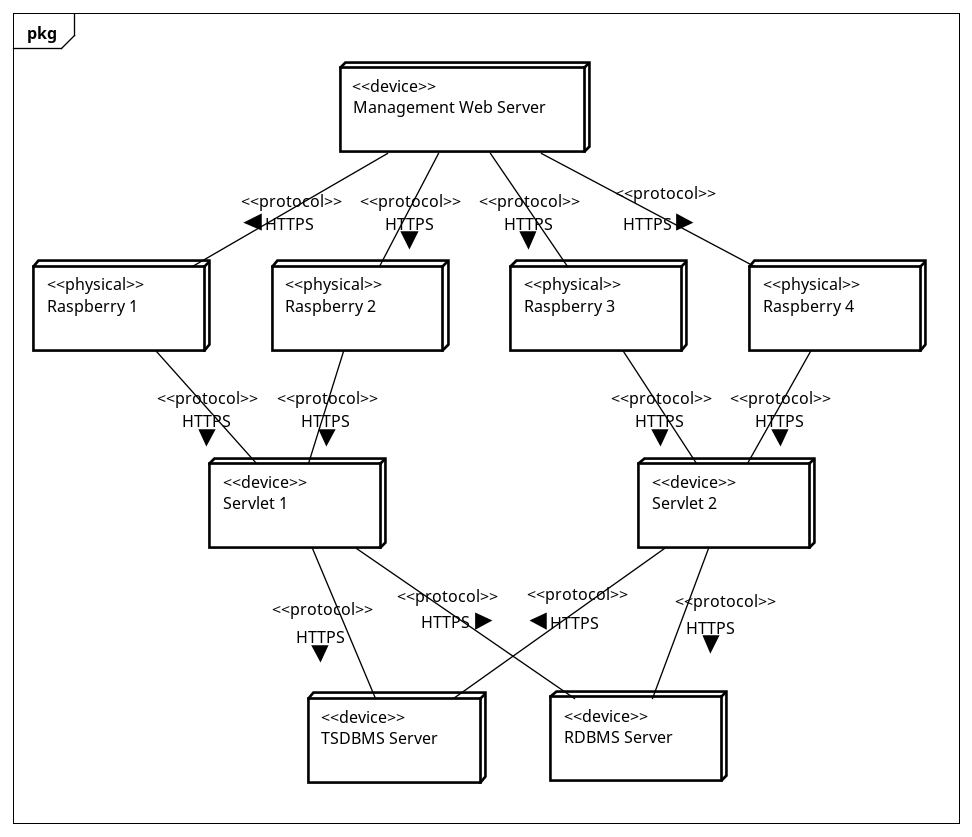
\includegraphics[scale=.45]{figure/Deployment_Diagram3v2.png}
	\caption{Diagramma di deployment (server distribuito con layer di smistamento) \label{DD LAYERED}}
\end{figure}


\section{Sicurezza}
Come evidenziato in fase di analisi dei requisiti, la sicurezza è un fattore critico per il successo del sistema.
Si rende quindi essenziale considerare la sicurezza già in fase di progettazione, in modo da minimizzare il numero e l'impatto delle eventuali vulnerabilità residue.
Per raggiungere questo scopo si agisce principalmente su due fronti: le comunicazioni di rete e il funzionamento interno dei servizi.

\subsection{Comunicazioni di rete}
Il primo aspetto di criticità è la modalità con cui avvengono le comunicazioni di rete, che costituiscono il fulcro del sistema.
Essendo il sistema pensato per funzionare sfruttando la rete Internet, occorre adottare opportune strategie per garantire autenticazione, riservatezza e integrità per ogni trasferimento dati.
Sono possibili anche varianti non basate su Internet, bensì su reti di tipologia differente.
La rete del sistema è suddivisibile in due macro-parti con caratteristiche diverse:
\begin{itemize}
 \item tra i Raspberry e la/le Servlet, caratterizzata da un elevata cardinalità e un ridotto traffico per singola connessione;
 \item tra la/le Servlet e il database, caratterizzata da un elevato volume di traffico su un singolo collegamento (o al limite poco più).
\end{itemize}
\paragraph{TLS}
Poiché le comunicazioni avvengono per design sfruttando interfacce REST e quindi il protocollo HTTP su TCP/IP, una prima possibilità è quella di adottare il protocollo TLS 1.2, la più recente versione di \textit{Transport Layer Security} (in futuro sarà possibile utilizzare le nuove versioni del protocollo con un aggiornamento software), che fornisce i servizi richiesti ed è lo standard del settore.
Ogni servizio sarà configurato in modo da accettare richieste solo con questo protocollo.
I dettagli sugli algoritmi crittografici e di hashing da utilizzare sono demandati all'implementazione, con la raccomandazione di consentire esclusivamente algoritmi sicuri e di disabilitare completamente quelli obsoleti.
Questa è la scelta che è stata effettuata per il sistema.
\paragraph{Rete ad hoc}
Una prima variante è quella di utilizzare una rete ad hoc separata da Internet.
Questa opzione, sebbene possibile, sarebbe probabilmente inutilmente costosa, in quanto richiederebbe la realizzazione di una nuova rete, senza possibilità di riutilizzare quella esistente.
Inoltre, la maggiore sicurezza derivante da questa architettura di rete appare ridondante, in quanto il protocollo TLS è sufficientemente sicuro da viaggiare su Internet senza rischi significativi.
Questa via potrebbe essere utile nel caso si scegliesse di utilizzare dispositivi embedded a capacità computazionale estremamente ridotta, al punto da non essere in grado di eseguire i calcoli crittografici necessari a TLS, oppure nel caso in cui il sistema (o parte di esso) fosse fisicamente collocato in zone isolate, dove non è stata portata connettività Internet cablata, oppure nel caso la città già disponga di una propria rete utilizzata per altri scopi (ad esempio telecamere di videosorveglianza).
\paragraph{VPN}
Come alternativa alla crittografia basata su TLS, si può valutare di trasmettere i dati all'interno di tunnel VPN.
Questa opzione potrebbe essere scelta per evitare l'implementazione della crittografia come parte di questo sistema, appoggiandosi ad un servizio di sistema (la VPN) già sviluppato da terzi.
Tuttavia, questa scelta richiederebbe un tunnel VPN per ogni Raspberry (o piccolo gruppo di Raspberry), con conseguente aumento del carico sulle servlet, quindi appare poco sensata per il collegamento dei Raspberry alla Servlet, mentre potrebbe essere più ragionevole per quello tra Servlet e database.

\subsection{Sicurezza dei servizi}
I vari componenti software saranno scritti utilizzando linguaggi di alto livello che prevengano vulnerabilità di tipo buffer overflow.
In questo modo il problema viene spostato sugli interpreti o le macchine virtuali che eseguono il codice (ad esempio la \textit{Java Virtual Machine} (JVM) nel caso di Java).
L'accesso ai servizi dovrà essere ristretto tramite opportune policy dei firewall, in modo da esporre solo i servizi strettamente indispensabili, restringendoli, dove possibile, anche in base agli indirizzi IP (ad esempio, il TS-DBMS dovrà essere accessibile solo dalla/e servlet, e non dai Raspberry o da Internet in generale).
\paragraph{Virtualizzazione}
La modalità di deployment distribuita precedentemente descritta contribuisce ad un maggiore isolamento dei servizi rispetto alla modalità centralizzata.
Utilizzando macchine virtuali single-purpose è possibile mitigare notevolmente l'impatto di un'eventuale intrusione, dal momento che la compromissione di un server non implicherebbe quella totale di tutto il sistema.
In questo modo i tempi di risposta e ripristino da parte dei sistemisti sarebbe ridotto.
\paragraph{Permessi di esecuzione e MAC}
I servizi devono poter funzionare, dove possibile, con privilegi di esecuzione ridotti (idealmente, mai con i privilegi di root).
In questo modo, la compromissione di un servizio non comporterebbe automaticamente un danno per tutto il sistema.
Come ulteriore opzione, è possibile implementare sul sistema politiche di \textit{Mandatory Access Control} (MAC), in modo da confinare ulteriormente i servizi ai soli permessi strettamente necessari alla loro esecuzione.
Questo non vale solo per i servizi realizzati nell'ambito di questo progetto, ma anche per quelli installati sul sistema operativo, necessari al suo funzionamento.
\paragraph{Permessi sul database}
In base al principio di privilegio minimo (\textit{least privilege}), è possibile creare più utenti sul database con privilegi diversi, utilizzati dai vari utenti (umani e non), ad esempio:
\begin{itemize}
 \item un utente ad uso delle istanze della servlet che può inserire record, ma non eliminare o modificare quelli esistenti;
 \item un utente utilizzato per il monitoraggio, che può eseguire query in sola lettura.
\end{itemize}
